\section{Evaluation}
\label{sec:evaluation}

We implement TD-Pipe on top of vLLM 0.5.3~\cite{vllm2024}.
We evaluate the effectiveness of TD-Pipe by comparing it with SOTA approaches and report the KV cache memory usage fluctuation during running.
Additionally, we conduct an ablation study to assess the impact of our proposed approaches.

\subsection{Experimental Setup}
\label{Setup}
\begin{table}[!t]
\caption{GPU Configurations}
\label{tab:gpus}
\centering
\resizebox{0.95\linewidth}{!}{
\begin{tabular}{c c c c c}
\hline
\textbf{  Device  }&  \textbf{   FP16 Tensor Core   } & \textbf{   Bandwidth   } & \textbf{   Memory   } & \textbf{   AllReduce   }\\ 
\hline \hline
L20 &  119.5 TFLOPS & 864 GB/s   &   48  GB      &   14.65 GB/s\\
A100 &  312 TFLOPS & 1,935 GB/s  &   80  GB      &   14.82 GB/s\\
\hline
\end{tabular}
}
\end{table}

\noindent\textbf{Node testbed.} 
Two multi-GPU nodes as in Table~\ref{tab:gpus} are employed.
One has 4 NVIDIA L20 GPUs (48GB) and another one has 4 NVIDIA A100 GPUs (80GB).
These two nodes all communicate through PCIe switch with a peak all-reduce bandwidth at 14.65 GB/s and 14.82 GB/s respectively.
Specifically, we use Pytorch$\sim$v2.3.1, vLLM$\sim$v0.5.3, CUDA$\sim$12.4, and NCCL$\sim$2.20.5.

\begin{table}[!t]
\caption{Model Specifications.}
\label{tab:models}
\resizebox{0.45\textwidth}{!}{
\begin{tabular}{ccccccc}
\hline
\textbf{Name}                        & \textbf{Parameters} & \textbf{Layers} & \textbf{Heads} & \textbf{Hidden Size} &\textbf{ Prec.} \\ \hline\hline
\multicolumn{1}{c}{Llama2-13B-chat} & 26GB & 40     & 40    & 5,120  & FP16       \\
\multicolumn{1}{c}{Qwen2.5-32B-Instruct} & 64GB & 64     & 40    & 5,120  & BF16     \\
Llama2-70B-chat                    & 140GB & 80     & 64    & 8,192  & FP16  \\ \hline
\end{tabular}
}
\end{table}
\noindent\textbf{Model setup.}
We choose Llama2~\cite{touvron2023llama2} and Qwen~\cite{qwen2025qwen25technicalreport} in different model sizes.
As detailed in Table~\ref{tab:models}, they are Llama2-13B-chat, Qwen2.5-32B-Instruct, and Llama2-70B-chat. For simplicity, we refer to them as 13B, 32B, and 70B in the following sections.
Notably, the 32B and 70B models use the group query attention (GQA) technique, which results in a smaller KV cache capacity for the same token count.

\begin{figure*}[htbp]
    \centering   
    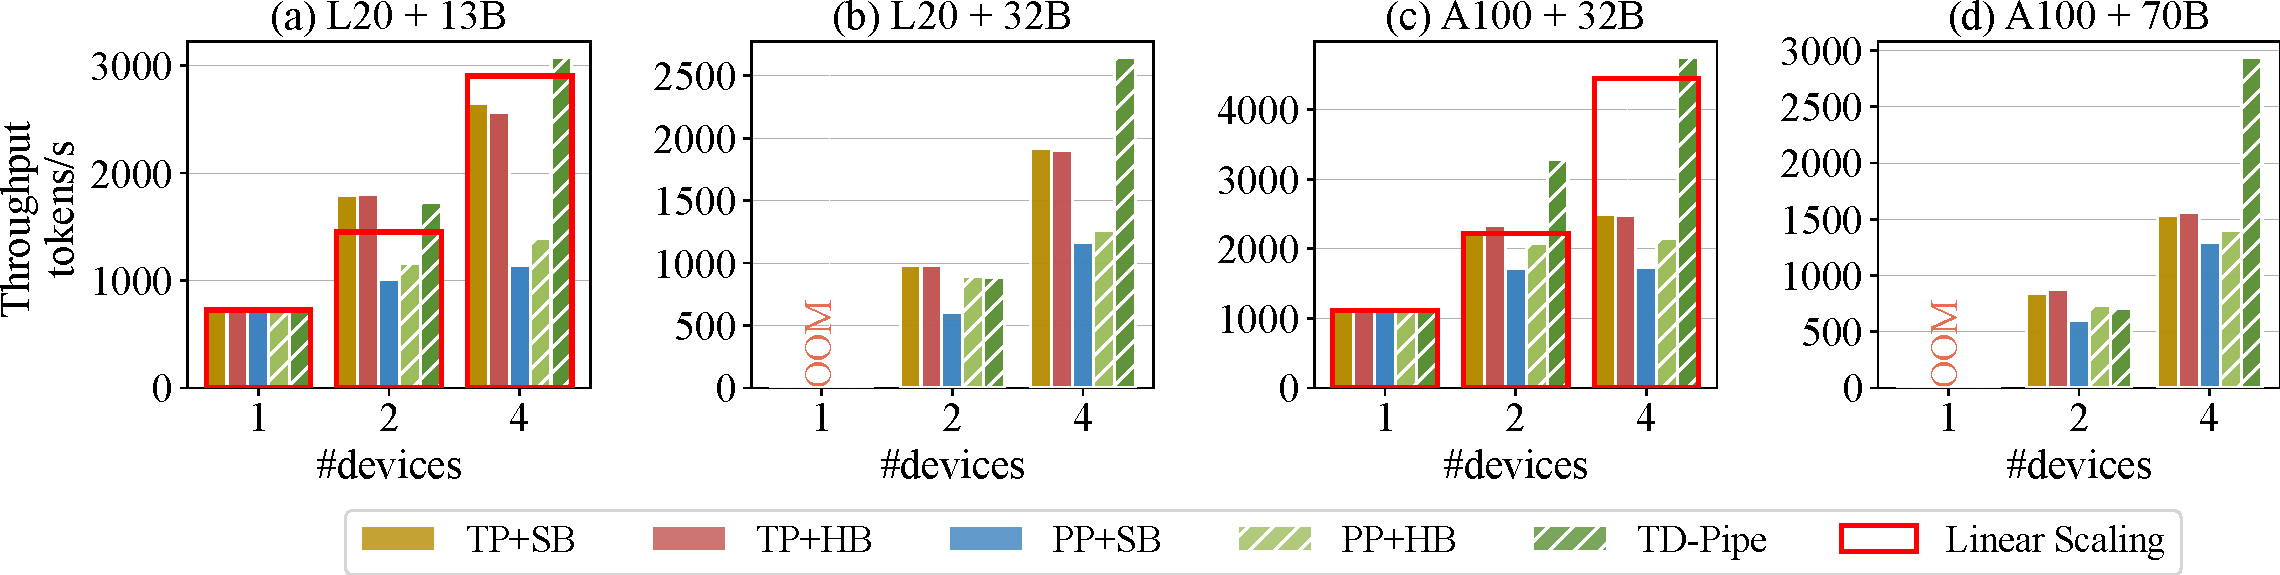
\includegraphics[width=0.9\linewidth]{graph/overall_perf.pdf}
    \vspace{-2pt}
    \caption{Overall performance.}
    \label{fig:overall-perf}
    \vspace{-10pt}
\end{figure*}
\noindent\textbf{Baseline Methods.}
We compare TD-Pipe with some recently released approaches implemented in vLLM~\cite{vllm2024}:
\begin{itemize}[leftmargin=*]
    \item \textbf{TP+SB}: The tensor parallel approach is integrated with separate batching. This method requires two All-reduce synchronizations in each transformer layer, and serves as the default approach in vLLM.
    \item \textbf{TP+HB}: The tensor parallel approach is integrated with hybrid batching, along with the chunked-prefill approach. This method also requires two All-reduce synchronizations in each transformer layer.
    \item \textbf{PP+SB}: The pipeline parallel approach is integrated with separate batching. This method requires limited communications but suffers from a severe bubble problem.
    \item \textbf{PP+HB}: The pipeline parallel approach is integrated with hybrid batching, along with the chunked-prefill approach. This method requires limited communications but still experiences the bubble problem.
\end{itemize}
Also, we employ the re-computation strategy where the KV cache of recently arrived requests will be freed once memory capacity is saturated, to deal with memory overflow issues.


\noindent \textbf{Dataset and Metrics.}
The popular conversation dataset, shareGPT V3~\cite{hfshareGPT}, is adopted in the evaluation.
The dataset contains around 53,000 samples, with each sample includes indefinite number of conversation rounds.
Following the benchmarking method used in vLLM, we filter input sentences with a length of less than 1024 tokens.
These input sentences are fed into the target models to generate new output sentences, constructing 86,612 input and output pairs.
For output length prediction training in the AI-based greedy prefill approach, 60\% of the samples are used as the training dataset, 20\% of the samples as the validation dataset, and all the other samples are used as the test dataset.
For performance evaluation, we randomly sample 5,000 input sentences as requests and use throughput (tokens/s) as the metric. 
Each execution of 5,000 requests takes around half an hour.

\subsection{Overall Performance Evaluation}

We compare TD-Pipe against baseline methods and present their overall throughput results for processing 5,000 input sequences.
Taking the ratio between memory capacity and model size into consideration, we select four node-model combinations: L20 + 13B, L20 + 32B, A100 + 32B, and A100 + 70B, and scale them from 1 to 4 GPUs.
We train output length predictor for these models respectively and report details in Section~\ref{sec:appeva1}.

Figure~\ref{fig:overall-perf} presents the throughput results, with the red box indicating the linear speed up.
In almost all cases, TD-Pipe presents advantages over other approaches, especially when the device number is 4.
For 4-device cases in all node-model configurations, TD-Pipe achieves up to 1.91$\times$ more throughput over TP+SB; 1.90$\times$ more throughput over TP+HB; 2.73$\times$ more throughput over PP+SB; and 2.21$\times$ more throughput over PP+HB.
Comparing PP+SB and PP+HB, it shows that the combination of hybrid batching and chunked-prefill approach can indeed optimize the pipeline parallelism by improving the inter-batch load balance. In contrast, TP+SB and TP+HB show fewer differences.

TD-Pipe demonstrates super-linear speedup as the number of GPUs increases from 1 to 4, largely outperforming other pipeline parallel approaches.
For example, when the GPU number scales from 2 to 4, the throughput of L20 + 32B grows 2.97$\times$.
When scaling from 2 to 4 GPUs, both the computing capability and the memory capacity are doubled.
On the one hand, the increased computing capability contributes to the speedup.
On the other hand, the increased memory capacity can be used for accommodating more KV cache and the computational intensity during the decode phase is largely improved.
Under the dual effects, TD-Pipe's throughput achieves super-linear improvement.
In comparison, the other two pipeline parallel approaches, PP+SB and PP+HB, show less improvement. This is because they are less impacted by memory capacity, and longer pipeline stages on more devices exacerbate their bubble problems.

Although TD-Pipe outperforms TP+SB and TP+HB in most cases, they can be constrained by various factors, i.e. memory capacity or coordination overhead.
Comparing L20 + 32B and A100 + 32B, we can first observe that A100 + 32B has significantly higher throughput than that of L20 + 32B, which aligns with the hardware specifications.
Additionally, we can also notice that the throughput ratio between TD-Pipe and TP methods varies between the two setups.
When performing with 4 GPUs, TD-Pipe achieves a performance improvement of 1.37$\times$ faster compared to TP+SB on the L20 node, while TD-Pipe is 1.90$\times$ faster than TP+SB on the A100 node.
This is related to many aspects, including the memory bandwidth, computing capability, memory capacity, and interconnection ability.
On the one hand, as shown in Table~\ref{tab:gpus}, the A100 is much more powerful than L20 in terms of both memory bandwidth and computing capability, while the interconnection ability is close.
Thus, TP+SB on the A100 node is more constrained by the interconnection, where TD-Pipe is much less reliant.
On the other hand, since all requests can be batched together 
using TP and requests are divided into multiple batches using PP, TP tends to achieve higher computational intensity than PP, while PP is more constrained by the memory capacity.
As a result, PP benefits more from the fact the A100 node's greater memory capacity.
Notably, since we record the overall throughput from the start of the first prefill to the finish of all decode batches, the execution tail of PP approach is less efficient compared to TP approach for its batch size is smaller. Nevertheless, our PP approach is still more effective than TP approach.


\subsection{KV Cache Memory Usage}


Figure~\ref{fig:memory_usage} illustrates the ratio of actual KV cache memory usage to the total allocated KV cache memory throughout the inference process, as the prefill and decode phases alternate over time.
Initially, KV cache memory usage increases continuously until the GPU memory approaches saturation, after which the system alternates between prefill and decode phases until all requests are completed.
For the prefill phase (in blue), the memory usage keep growing.
For the decode phase(in yellow), its memory usage always grows, fully occupied, and then begins to decline.
This is because new KV cache will be generated and some requests complete in the decode phase.
It is noted that the memory usage is only shortly occupied and it can illustrate the AI-based greedy prefill is effective.
\begin{figure}[htbp]
    \centering    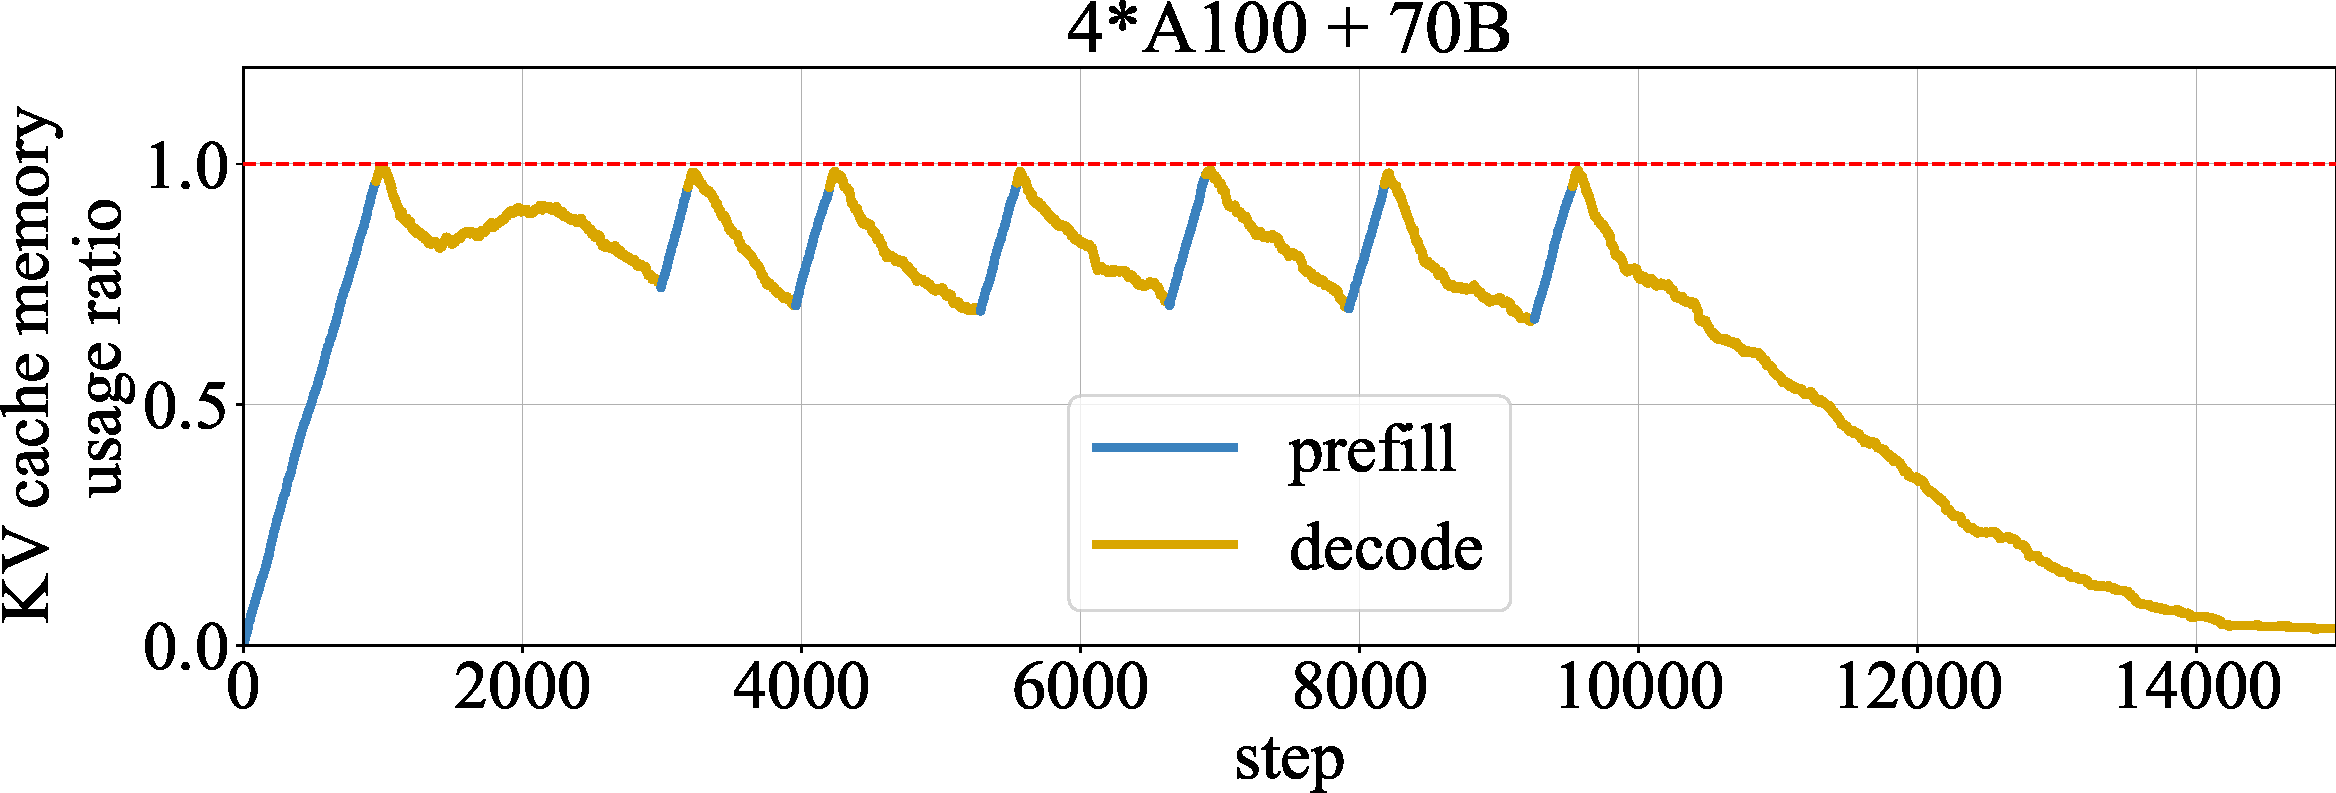
\includegraphics[width=0.9\linewidth]{graph/memory_usage.pdf}
    \vspace{-10pt}
    \caption{The KV cache memory usage fluctuation.}
    \label{fig:memory_usage}
    \vspace{-5pt}
\end{figure}


\subsection{Ablation Study}
This section illustrates how each approach impacts TD-Pipe.

\subsubsection{Approach-1: AI-based Greedy Prefill}
\label{sec:appeva1}

\begin{figure}[htbp]
    \centering    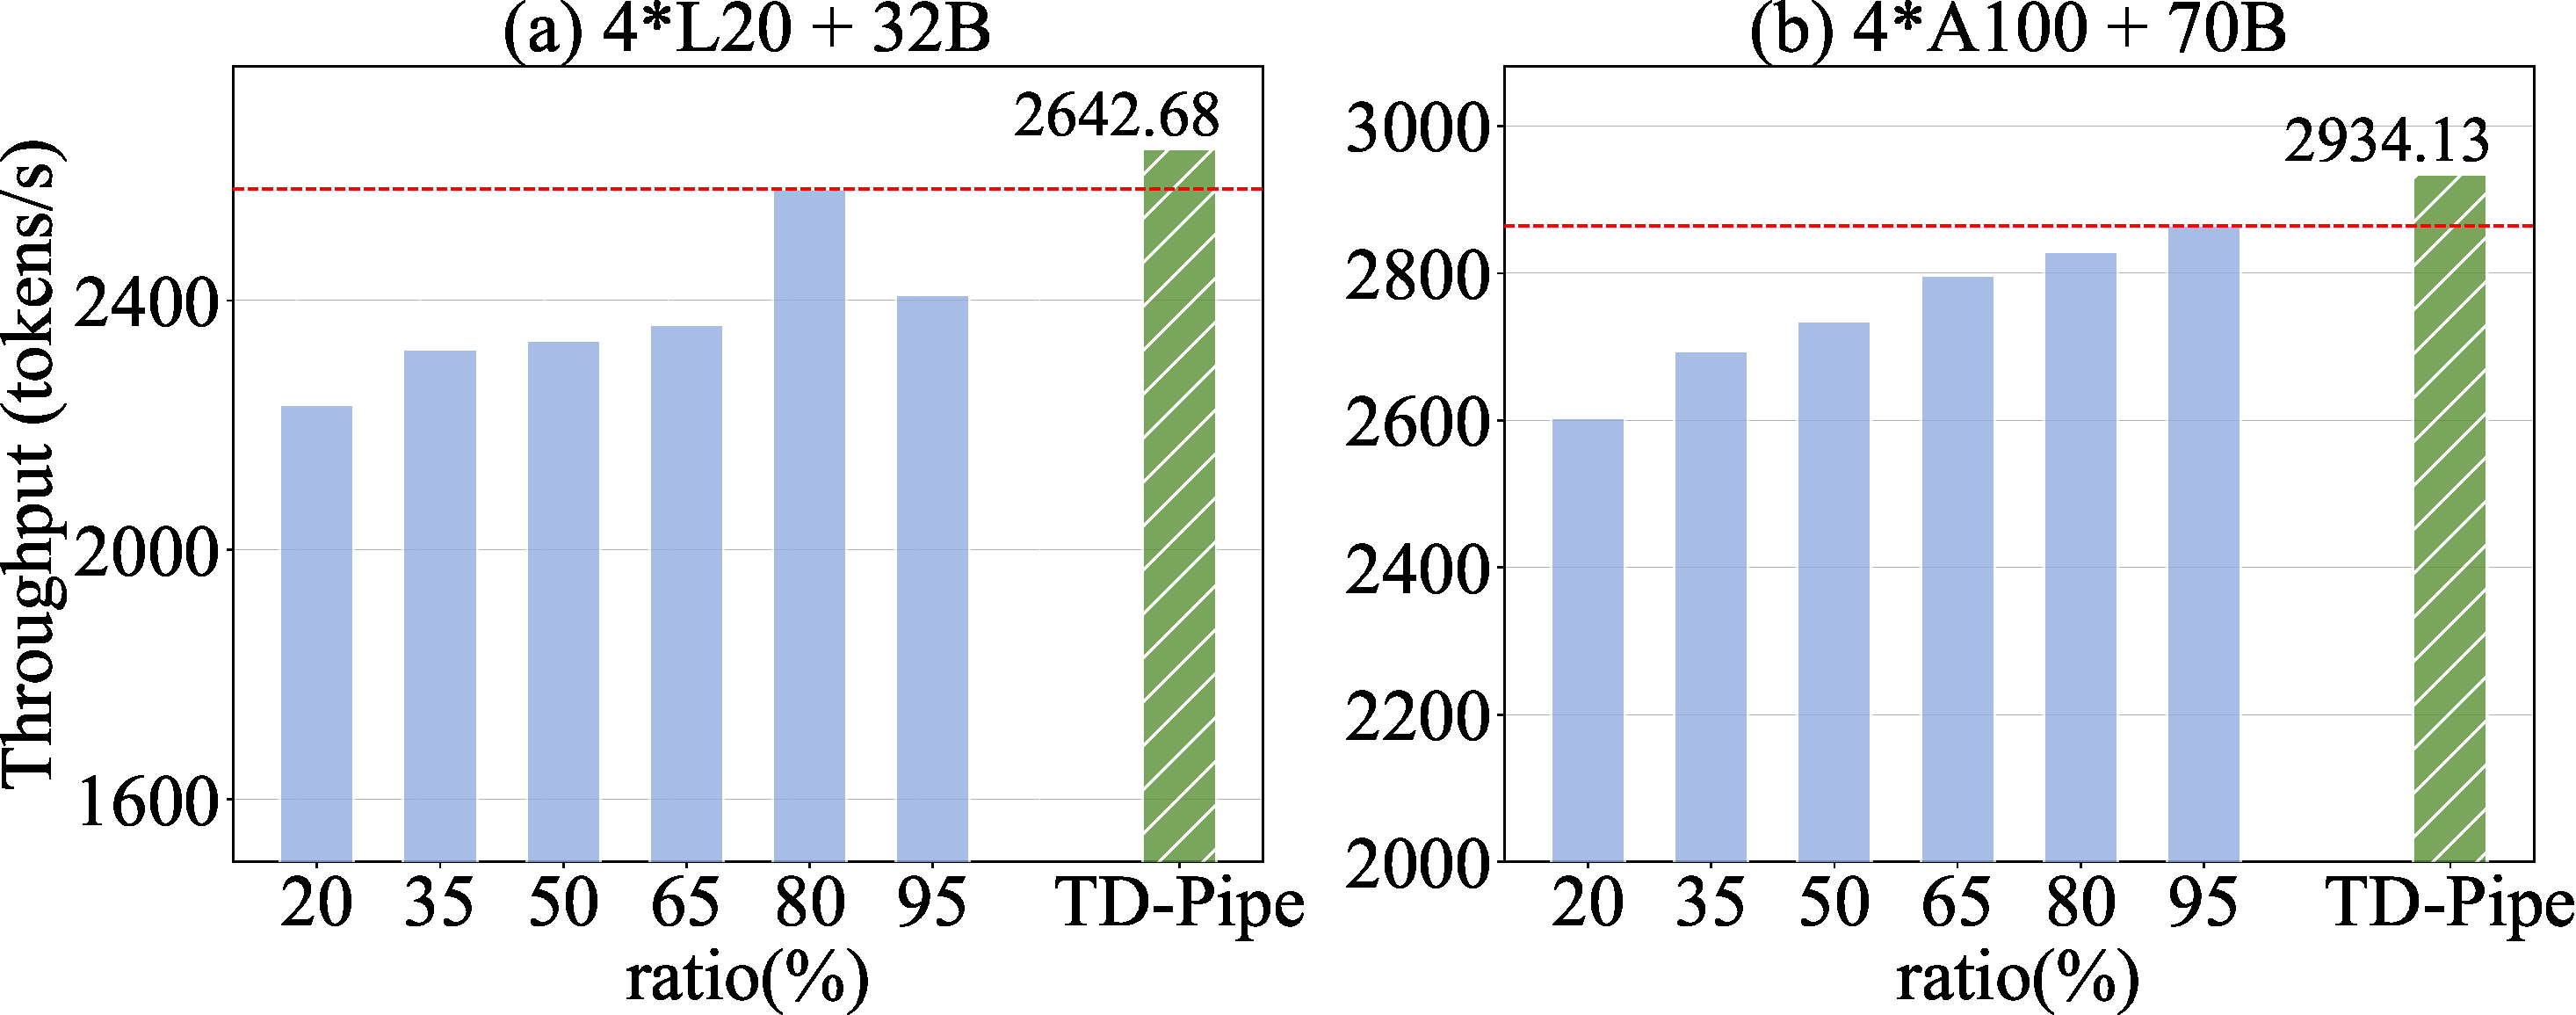
\includegraphics[width=0.9\linewidth]{graph/prefill-to-decode.pdf}
    \vspace{-10pt}
    \caption{Ablation study for prefill-to-decode switching.}
    \label{fig:prefill-to-decode}
\end{figure}
To demonstrate how effective the AI-based greedy prefill can determine the timing for switching from prefill to decode, we design a hyperparameter called the KV cache occupancy ratio to replace the AI-based greedy prefill approach.
For example, when we set this ratio as 50\%, the prefill will switch to decode once 50\% KV cache blocks are occupied.
Figure~\ref{fig:prefill-to-decode} shows the throughput results, demonstrating that our approach outperforms all other manually selected switching points.
For the hyperparameter approach, it requires human experience and numerous experiments.
This result illustrates that our AI-based greedy prefill approach can determine a fairly good switching point, and it can dynamically fit the constantly changing requests and diverse hardware configurations.  


Additionally, we report the prediction accuracy of the output length predictor.
The predictor is trained and deployed for each LLM model in FP16 precision. 
When predicting the length range of a single request, their accuracies are 0.5214, 0.5805, and 0.5234 for 13B, 32B, and 70B models, outperforming random guessing. 
Notably, single request's prediction accuracy can partially reflect its effectiveness in our scenario, while the accuracy of accumulated length prediction is more relevant.
Since some predictions may be overestimated while others are underestimated, the accumulated prediction accuracy can be smoothed out and better reflects the total KV cache size.
Therefore, as shown in Figure~\ref{fig:error}, we group samples in test set with different request numbers and evaluate the accumulated prediction error of each group.
The accumulated error is acquired by accumulating and averaging the relative difference between the predicted total length and the actual total length in all groups.
When the number of requests is large, the accumulated error becomes sufficiently small.
For example, when predicting the total output lengths of 256 requests, there are only 3.25\%, 6.18\%, and 2.84\%  errors for 13B, 32B, and 70B models.


\begin{figure}[htbp]
    \centering    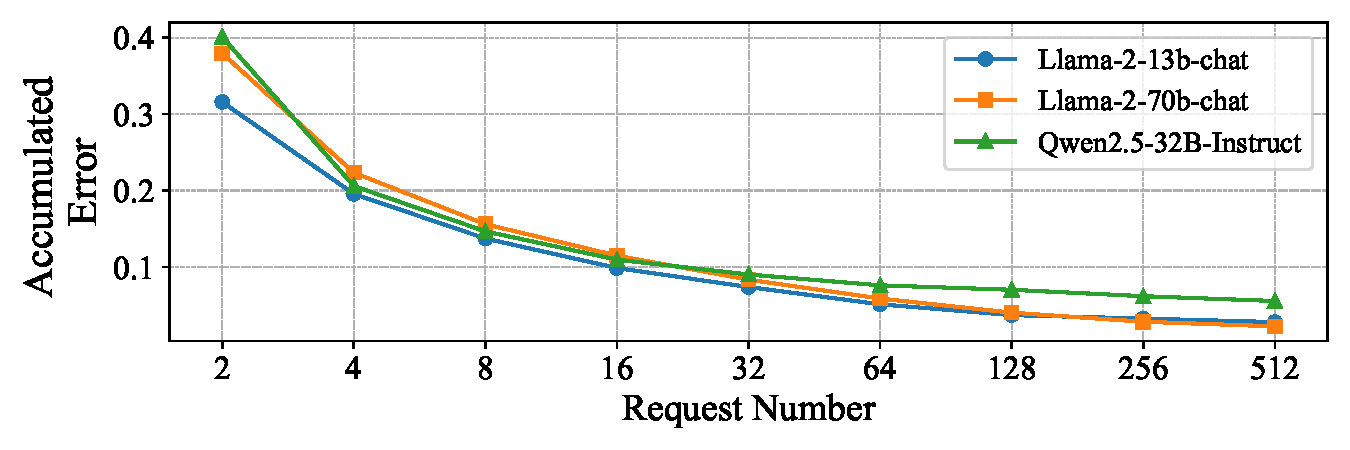
\includegraphics[width=0.9\linewidth]{fig/error.pdf}
    \vspace{-10pt}
    \caption{The accumulated error of varied request number.}
    \label{fig:error}
\end{figure}



Furthermore, we evaluate the overhead introduced by the predictor. For 5,000 requests, the predictor takes 1,418.861 ms on the L20 node and 833.695 ms on the A100 node.
In the experiments described in Section~\ref{Setup}, the shortest total processing times observed are 929 seconds on the L20 and 602 seconds on the A100.
Given that the predictor’s execution time remains consistent across all models, it contributes less than 0.153\% of the total processing time on the L20 and 0.138\% on the A100, confirming that the overhead is negligible.


\subsubsection{Approach-2: Inter-batch Work Stealing}

\begin{figure}[h]
    \centering    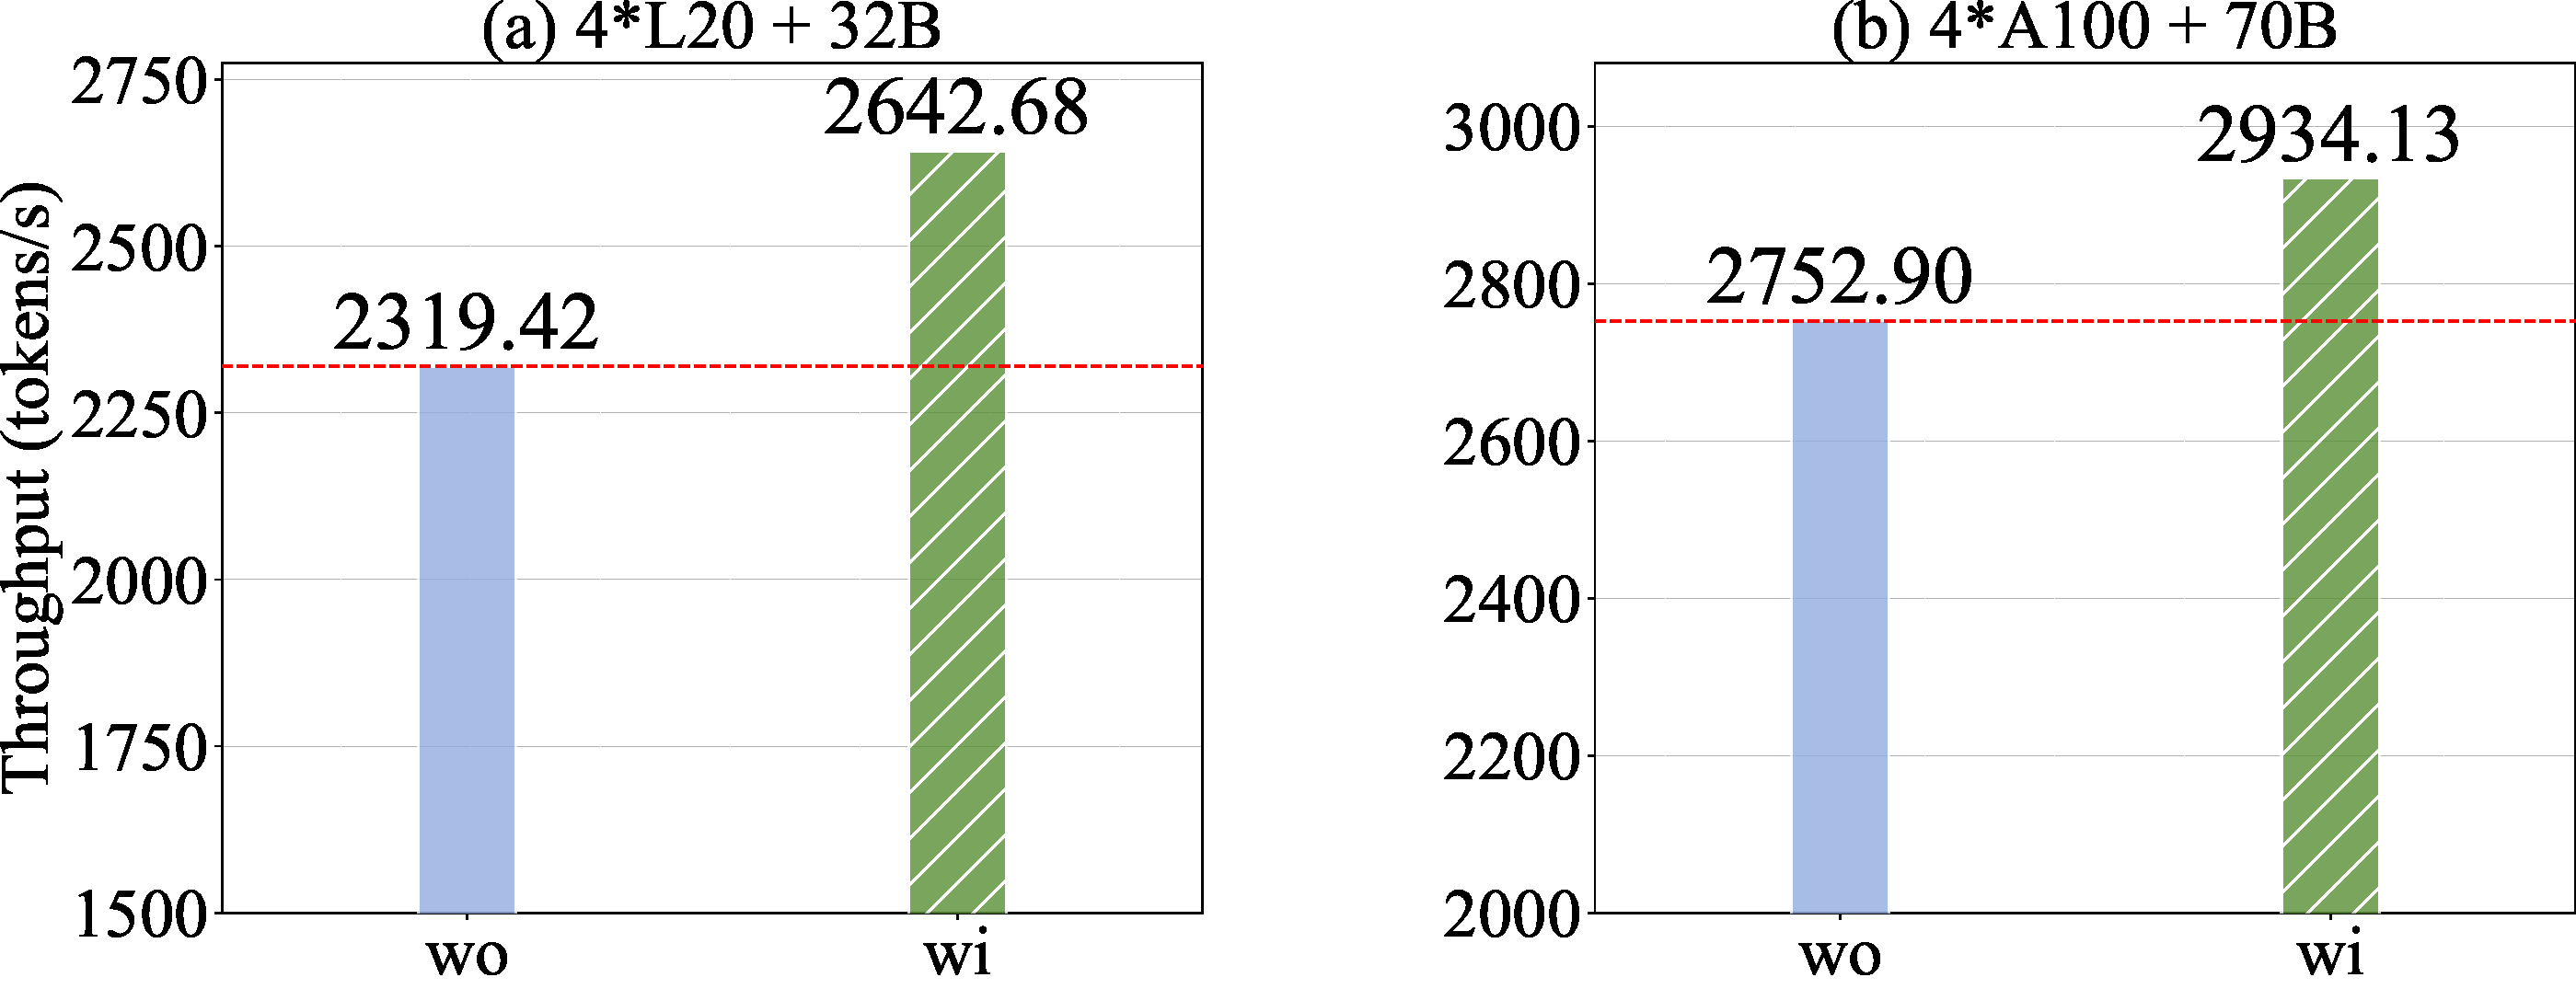
\includegraphics[width=0.9\linewidth]{graph/approach2.pdf}
    \vspace{-10pt}
    \caption{Ablation study for the decode batch load balance.}
    \label{fig:approach2}
\end{figure}

We report throughput results with (\textbf{wi}) or without (\textbf{wo}) the inter-batch work stealing approach in Figure~\ref{fig:approach2}.
The load balance scheduling at the timing for switching from prefill to decode is still kept and only the dynamic balance during the decode phase is removed.
L20 + 32B and A100 + 70B have 1.14$\times$ and 1.07$\times$ throughput improvement after activating our inter-batch work stealing approach, validating its effectiveness.

\subsubsection{Approach-3: Spatial Temporal Intensity Comparison}

\begin{figure}[h]
    \centering    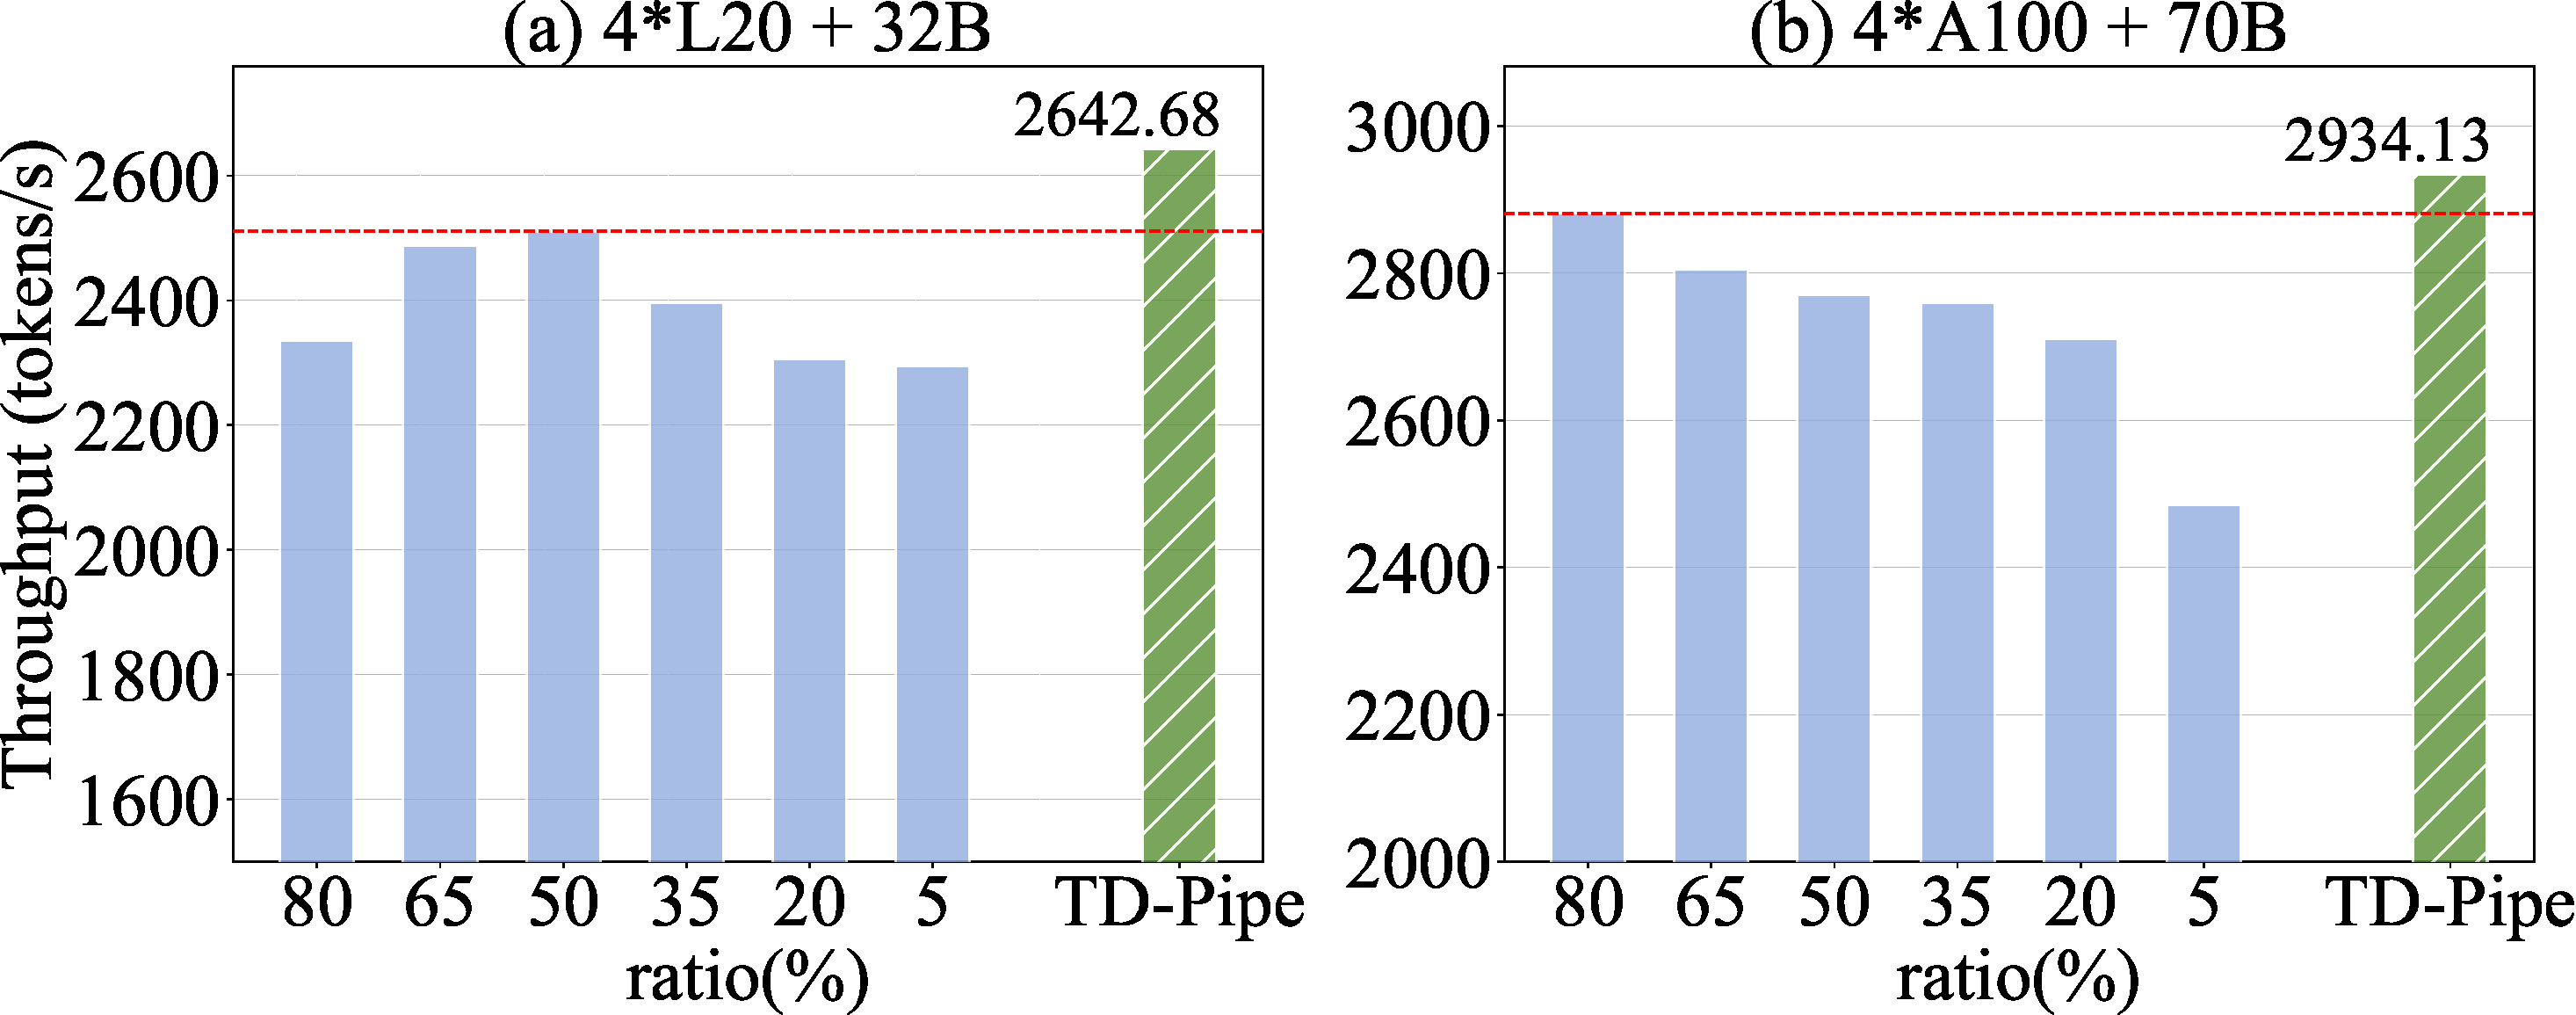
\includegraphics[width=0.9\linewidth]{graph/decode-to-prefill.pdf}
    \vspace{-10pt}
    \caption{Ablation study for decode-to-prefill switching.}
    \label{fig:decode-to-prefill}
\end{figure}

Like evaluating the AI based greedy prefill approach, we introduce a hyperparameter called the request finish ratio to replace the spatial temporal intensity comparison approach.
For example, if this ratio is set to 50\%, the decode phase will switch to prefill once 50\% of the requests have completed.
In Figure~\ref{fig:decode-to-prefill}, the manually selected points perform well even when the ratio is somewhat extreme, due to the large memory capacity in these cases.
In comparison, the spatial temporal intensity comparison approach consistently achieves the highest throughput, illustrating its effectiveness.



